%-------------------------------------------------------------------------------
% MODELISATION
%-------------------------------------------------------------------------------
\subsubsection{Modélisation}

Le problème du voyageur de commerce peut se modéliser de la manière
suivante~:


on se donne un graphe complet $K_n=(X,E)$ et on note $c_{ij}$ le poids
de l'arête $\{i,j\}$.
\begin{equation}
\begin{cases}
min \sum_{\{i, j\} \in E} c_{ij}.x_{ij} \\
\sum_{i=0}^n \sum_{j=0}^n x_{ij} = 1 \\
\forall (S, \bar{S}) \sum_{i \in S, j \in \bar{S}} x_{ij} \geq 1 \\
x_{ij} \in \{0, 1\} \\
\end{cases}
\end{equation}

%-------------------------------------------------------------------------------
% FORMULAS
%-------------------------------------------------------------------------------
\subsubsection{Formules de programmation dynamique}

On note $C(S,i)$ la longueur d'une plus courte chaîne du sommet $0$ au
sommet $i$ qui passe une et une seule fois par tout sommet de $S$ et
qui n'utilise pas de sommet non dans $S$ autre que $i$. On a ainsi les
formules suivantes pour le problème du voyageur de commerce~:

\begin{equation}
\begin{cases}
C[S][i] = poids[0][i] \text{si S ne contient que $0$} \\
C[S][i] = min_{k \in S - \{ 0 \}} \{ C[S- \{ k \}][k] + poids[k][i]  \}
\end{cases}
\end{equation}

Le principe appliqué à un chemin/cycle (il y a autant de chemins que de
sommets moins un) peut être résumé sur le schéma présenté ci-dessous.

\begin{figure}[!ht]
\begin{center}
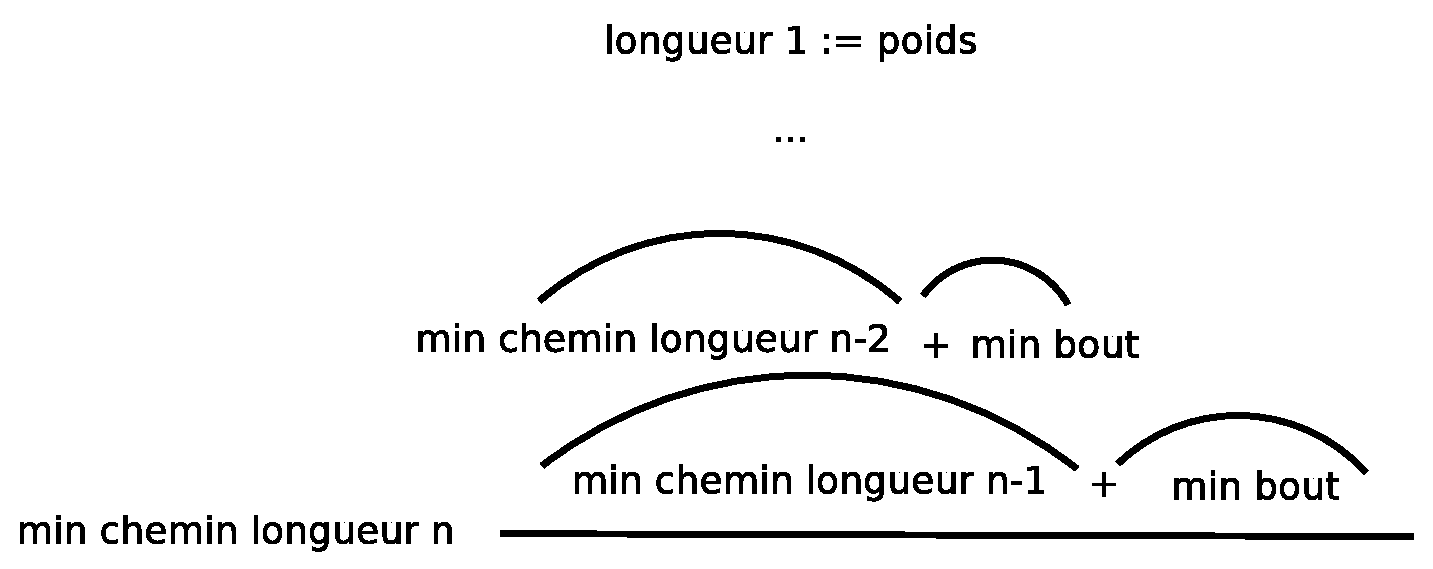
\includegraphics[height=5cm]{../images/tspDyn.eps}
\end{center}
\caption{Exemple de calcul d'un chemin pour le tsp en programmation dynamique.}
\end{figure}

%-------------------------------------------------------------------------------
% ALOGORITHM
%-------------------------------------------------------------------------------
\subsubsection{Principe de l'algorithme}

Nous proposons l'algorithme suivant pour une programmation dynamique
du TSP.

\begin{algorithm}[!ht]
\caption{Programmation dynamique pour le TSP}
\label{Dyntsp}
\begin{algorithmic}[1]
\REQUIRE une matrice de poids, un ensemble de $n$ sommets
\FOR{chaque sous-ensemble $S$ commençant par $0$}
\IF{$|S| = 2$}
\FOR{$i$ de $0$ à $n-1$}
\STATE C[S][i] := poids[0][i]
\ENDFOR
\ELSE
\FOR{$i$ de $0$ à $n-1$}
\FOR{tous les $k$ $\notin$ $S - \{ 0 \}$}
\STATE C[S][i] := $\min$ $\{$ C[$S - \{ k \} $][k] + poids[k][i] $\}$
\ENDFOR
\ENDFOR
\ENDIF
\ENDFOR
\STATE retourner $\min$ $\{$ C[S][i] + poids[i][0] $\}$ avec $|S| = $
(nombre de sommets - 1)
\end{algorithmic}
\end{algorithm}

%-------------------------------------------------------------------------------
% IMPLEMENTATION
%-------------------------------------------------------------------------------
\subsubsection{Implémentation en C++}

%-------------------------------------------------------------------------------
% COMPLEXITÉ
%-------------------------------------------------------------------------------
\subsubsection{Complexité}

La complexité théorique d'un tel algorithme est de $O(n^2.2^n)$.

%-------------------------------------------------------------------------------
% TESTS
%-------------------------------------------------------------------------------
\subsubsection{Jeux de tests}
Nous mesurons ici une moyenne du temps d'exécution sur 5 tests en
faisant varier le nombre de sommets à parcourir. Nous obtenons les
résultats présentés ci-dessous.

\begin{figure}[ht]
% LEFT-HAND SIDE
\begin{minipage}[b]{0.5\linewidth}
\centering
\begin{tikzpicture}[scale=0.9]
    \begin{axis}[title=Jeux de tests pour le TSP, xlabel= nombre de
        villes parcourues, ylabel= temps d'exécution]
      \addplot
        table[col sep=comma]{../charts/tspdyn.csv};
        %\legend{exécution du tsp}
    \end{axis}
\end{tikzpicture}
\caption {Courbe des temps d'exécution pour TSP}
\end{minipage}
% RIGHT-HAND SIDE
\hspace{0.5cm}
\begin{minipage}[b]{0.5\linewidth}
\centering
\begin{tabular}{|c|c|}
\hline
Sommets & t moyenne en ms\\
\hline
2 & $\simeq 0$\\
\hline
5 & 2\\
\hline
7 & 15\\
\hline
9 & 137\\
\hline
11 & 1151\\
\hline
13 & 8575\\
\hline
15 & 58109\\
\hline
\end{tabular}
\caption {Tableau des temps d'exécution pour TSP}
\end{minipage}
\end{figure}
